% Chapter Template

\chapter{Analysis of Results} % Main chapter title

\label{Analysis} % Change X to a consecutive number; for referencing this chapter elsewhere, use \ref{ChapterX}

\lhead{Chapter 5. \emph{Analysis of Results}} % Change X to a consecutive number; this is for the header on each page - perhaps a shortened title

Given the good performance of the \textsc{LangID} and \textsc{LangF} models presented in Chapter~\ref{Stage1}, it would be useful to further investigate these models to find out where good performance comes from. This may suggest further improvements and directions for future work. This analysis will take place in several parts. First, I will explore how much training data is necessary for a well-performing model, and to what extent out-of-language data can substitute for it. Then\todo{will this stay?}, I will investigate the effect that using language representations has on the quality of results. Finally, I will analyze the internal structure of the models' learned embeddings.

%the importance of training data will be explored, in order to determine how much in-language data is necessary for the Chapter~\ref{Stage1} approaches to succeed. In addition to the weighted finite state transducer-based baseline used in Chapter~\ref{Stage1}, results will be compared to the output of monolingually-trained sequence-to-sequence models. 

\section{Training Data}
One of the challenges of low resource NLP is to build systems that perform well with less training data. The results in Chapter~\ref{Stage1} showed that multilingual data can be helpful in a sequence-to-sequence model-based approach to g2p. This raises an important question: how much of an effect does multilingual training have on the quality of results? That is, how do monolingually trained networks perform on the same test data?

%\begin{itemize}
%\item How much training data is necessary for a sequence-to-sequence model to perform well in this domain? At some quantity of data, it probably becomes impossible to train a monolingual model. What is this quantity, and does vary by language?
%\end{itemize}

%\subsection{Monolingual Models}
In order to answer this question, I implemented monolingual g2p models for a subset of the languages present in the \textsc{WikiPronounce} corpus. Languages were included if they met these conditions:

\begin{itemize}
\item Words for the language are present in the training and validation data used for \textsc{LangID-All} and \textsc{LangF-All}.
\item The language's test set in \textsc{WikiPronounce} contains a full 200 words.
\end{itemize}

This leaves 83 languages to build monolingual g2p models for. Each monolingual model was trained on the same training samples as were present for its language in the training data for \textsc{LangID-All} and \textsc{LangF-All}. The architecture and training conditions are identical to those used for the \textsc{LangID} and \textsc{NoLangID} models, except that the batch size was determined automatically from the training size for each language because it is difficult to train on small batch sizes. The batch sizes used are listed in Figure~\ref{table:batch}. Because each individual network is monolingual, it is not necessary to add a token or feature identifying the language for any of these models. Translations were performed using a beam width of 5, rather than the 100 used in Chapter \ref{Stage1}, because it is inefficient to compute for so many models and because WER 100 is not necessary for the analysis. These monolingual networks are then compared to the output of \textsc{LangID-All}\footnote{One could also compare results to \textsc{LangF-All}. However, the \textsc{LangF-All} results are very similar, so the plots are omitted for he sake of brevity.}. Results were recomputed for this model with a beam width of 5 to match the monolingual conditions.

The benefit from training multilingually instead of monolingually is shown in Figures \ref{figure:perimprove} and \ref{figure:werimprove}. On both metrics, it can be seen that the improvement from multilingual training is very large for the languages with the least training data. This benefit gradually shrinks, and the monolingual result often exceeds the multilingual one by the time the training size reaches about 5000.

\begin{table}
\begin{tabular}{lrr}
\toprule
{} &        PER &        WER \\
\midrule
Monolingual  &  37.421928 &  63.560241 \\
\textsc{LangID-All} &  17.028795 &  48.518072 \\
\bottomrule
\end{tabular}
\caption{Average per-language performance of monolingually-trained networks and \textsc{LangID-All} on }
\end{table}

\begin{table}
\centering
\small
\begin{tabular}{|c|c|}
\hline
Training Size & Batch Size \\
\hline
$\geq 5000$ & $16$ \\
$2000 \leq x < 5000$ & $8$ \\
$4 \leq x < 2000$ & $4$ \\
$<4$ & Same as training size \\
\hline
\end{tabular}
\caption{Batch sizes used for monolingual models}
\label{table:batch}
\end{table}

\begin{figure}
\begin{center}
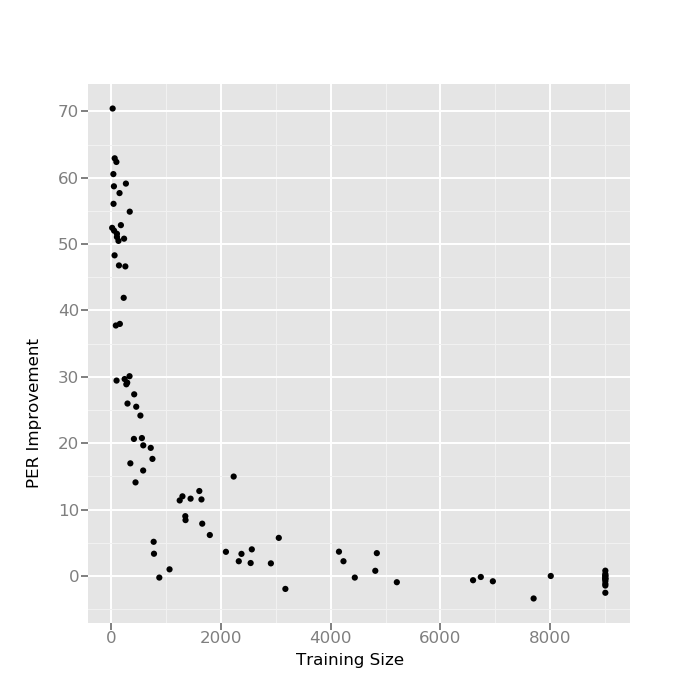
\includegraphics[scale=0.75]{Figures/perimprove}
\end{center}
\caption{Phoneme Error Rate by language for the monolingual g2p models.}
\label{figure:perimprove}
\end{figure}

\begin{figure}
\begin{center}
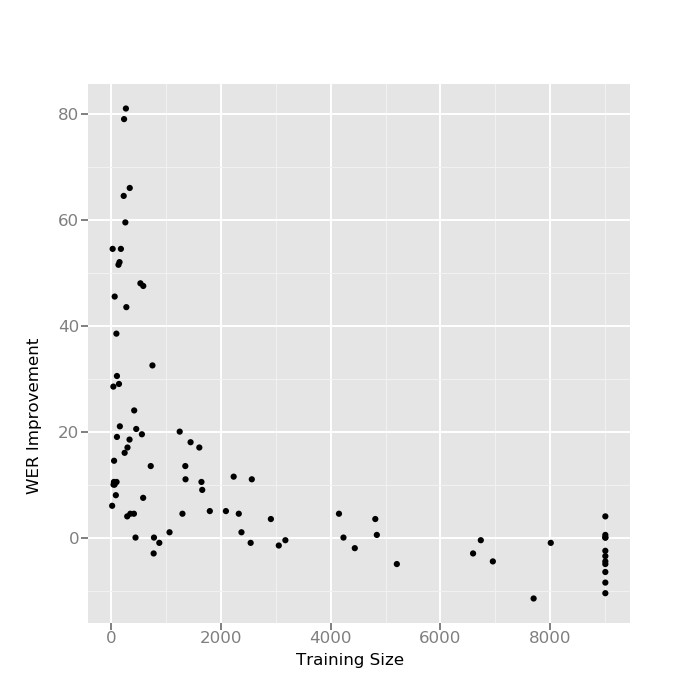
\includegraphics[scale=0.75]{Figures/werimprove}
\end{center}
\caption{Phoneme Error Rate by language for the monolingual g2p models.}
\label{figure:werimprove}
\end{figure}

%\subsection{Necessity of Training Data}
%The results of these monolingual networks are shown in Figures \ref{figure:mono-per} and \ref{figure:mono-wer}. The same basic trend can be seen for both metrics: there is an elbow in the error rate curves when the training size is somewhere between 2000 and 4000 samples, although it is possible this can be partially explained by other factors, such as higher resource languages having more standardized systems of orthography. The effect of quantity will be explored in more depth in\todo{make this thing}.

%It is not clear, however, how much of this improvement is due to the additional training data and how much could be the result of other factors. One plausible hypothesis is that the data available for the lower resource languages in the set is noisier, and therefore it is more difficult for the model to learn the grapheme-phoneme correspondences for those languages. It could also be possible that higher resource languages, given their higher prestige, are likely to have more 

%\begin{figure}
%\begin{center}
%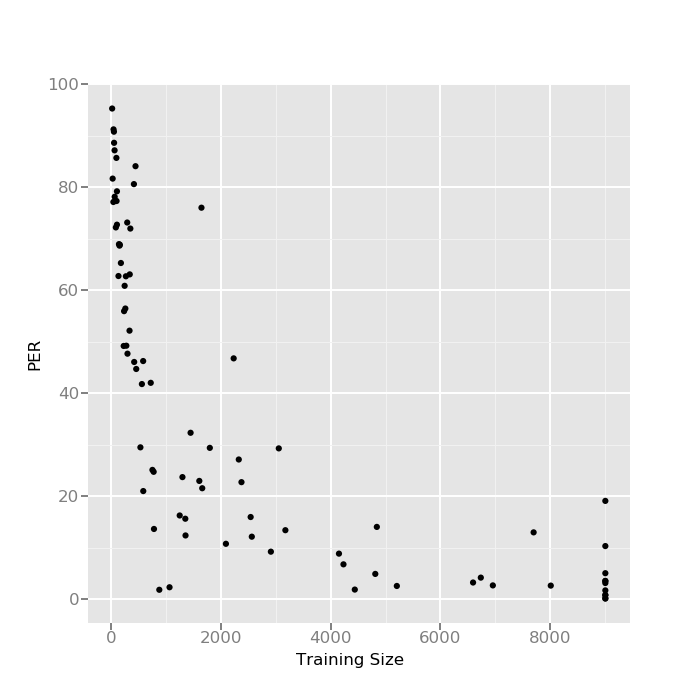
\includegraphics[scale=0.75]{Figures/mono-per}
%\end{center}
%\caption{Phoneme Error Rate by language for the monolingual g2p models.}
%\label{figure:mono-per}
%\end{figure}

%\begin{figure}
%\begin{center}
%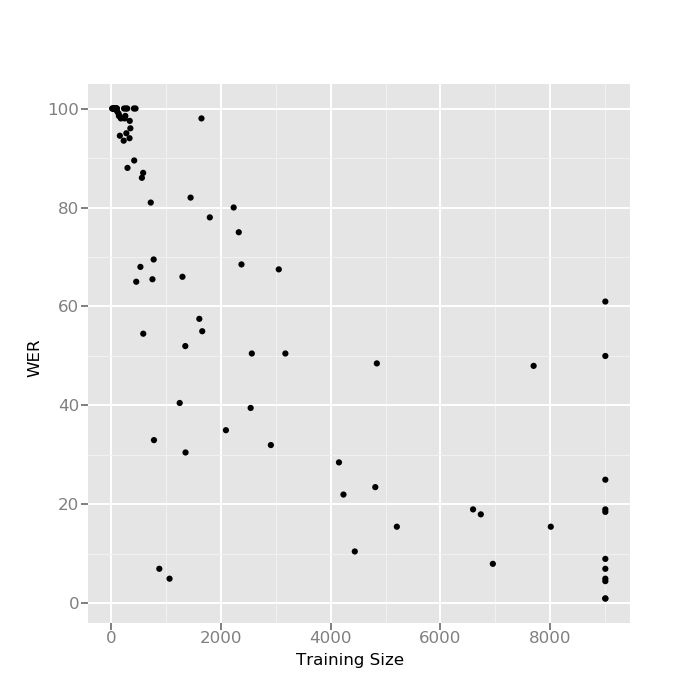
\includegraphics[scale=0.75]{Figures/mono-wer}
%\end{center}
%\caption{Word Error Rate by language for the monolingual g2p models.}
%\label{figure:mono-wer}
%\end{figure}

%Given the clear benefit\todo{this needs to change a little bit, and also I need to get the results} that the multilingually-trained models have on languages with less training data, it would be useful to explore the performance of these models further. Results for the \textsc{LangF-All} and \textsc{LangID-All} models results on the languages used in the previous section are reported below: PER results are shown in Figure \ref{figure:per-by-lang}, WER results are shown in Figure \ref{figure:wer-by-lang}, WER 100 results are shown in Figure \ref{figure:wer100-by-lang}.

%The same basic trend can be seen with all three of these error metrics: among languages with very few training samples (less than about 1000), there is a wide diversity of outcomes: for many of these low-data languages, the models perform very well, and for others very poorly. As the quantity of in-language data increases, results improve. For PER and WER 100 (and to a lesser extent WER), there is an ``elbow'' at around 2000 training samples. Above 2000 samples, performance of the multilingual models is more stable: the worst-performing ones with that much data have PER and WER 100 scores of around 20\%\footnote{The relationship between PER and WER is not consistent across languages because some languages have longer words than others. This is mitigated in WER 100 because the system has so many chances to guess the word correctly.}.

\begin{figure}
\centering
\begin{tabular}{lrrrrrr}
\toprule
{} & \multicolumn{3}{l}{\textsc{LangID-All}} & \multicolumn{3}{l}{\textsc{LangF-All}} \\
{} &        PER & WER & WER 100 &       PER & WER & WER 100 \\
\midrule
bul  &       1.24 &  8.00 &    1.00 &      1.08 &  6.00 &    1.00 \\
deu  &       5.78 & 33.50 &    5.50 &      4.82 & 28.50 &    4.00 \\
eng  &      21.66 & 71.50 &   14.00 &     18.48 & 63.50 &   12.00 \\
epo  &       2.71 &  3.00 &    0.50 &      3.26 &  5.50 &    1.00 \\
fra  &       4.29 & 24.00 &    2.00 &      3.33 & 18.50 &    1.50 \\
hbs  &       0.06 &  0.50 &    0.00 &      0.12 &  1.00 &    0.00 \\
hun  &       1.94 & 11.50 &    0.00 &      1.55 &  9.00 &    0.50 \\
kat  &       0.11 &  1.00 &    0.00 &      0.11 &  1.00 &    0.00 \\
lit  &       1.19 &  9.50 &    0.50 &      1.10 &  8.50 &    1.50 \\
pol  &       3.21 & 18.50 &    1.50 &      3.40 & 20.50 &    1.00 \\
rus  &      11.73 & 56.50 &    4.00 &     11.35 & 54.50 &    4.50 \\
\midrule
Mean &       4.90 & 21.59 &    2.64 &      4.42 & 19.68 &    2.45 \\
\bottomrule
\end{tabular}
\caption{Results of \textsc{LangID-All} and \textsc{LangF-All} models on languages with 9000 training samples and 200 test samples}
\label{figure:big-lang-results}
\end{figure}

%\section{Multilingual Training}
%The clearest innovation of the \textsc{LangID} and \textsc{LangF} models is that they rely on multilingual training. Although I previously showed that this leads to improvements relative to a non-neural baseline, it would additionally be useful to compare the results of the \textsc{LangID} and \textsc{LangF} models against monolingually-trained networks in order to directly test the effect of training on out-of-language data in addition to in-language data.

%\subsection{Data}
%I trained monolingual models for the 84 languages which have a full 200-word test set in \textsc{WikiPronounce}\footnote{It would also have been to train monolingual models for languages with smaller test sets. However, they were excluded because error metrics are more prone to random variation on smaller dataset.}. The number of training samples for these varies from 9, for Medieval Spanish, to 9000, for various high-resource languages. Statistics describing these languages are shown in Table\todo{make} and results of \textsc{LangID-All} and \textsc{LangF-All} on this subset of the test languages is shown in Table\todo{make}.

%\subsection{Training}
%Each model was trained on the same training samples as were present for its language in the training data for \textsc{LangID-All} and \textsc{LangF-All}. The architecture and training conditions are identical to those used for the \textsc{LangID} and \textsc{NoLangID} models, except that the batch size was determined automatically from the training size for each language\todo{how?}. This was necessary because it was impossible to train small datasets with large batch sizes, and larger datasets performed better with larger batch sizes. Because each individual network was monolingual, it was not necessary to add a token or feature identifying the language for any of these models.

%\begin{figure}
%\begin{center}
%\includegraphics[scale=0.7]{Figures/monolingual-per}
%\end{center}
%\caption{Phoneme error rate for monolingually-trained low resource languages}
%\label{figure:lr-per}
%\end{figure}

%\subsection{Results}
%As the results in Figure \ref{figure:lr-per} show, performance was quite poor in the monolingual low-resource case. However, improvement was markedly better when using the multilingually-trained model, as is shown in Figure \ref{figure:multi-improve}.\todo{a table with complete results would be better. So would maybe be training the thing for more languages}

%\begin{figure}
%\begin{center}
%\includegraphics[scale=0.7]{Figures/multi-improve}
%\end{center}
%\caption{Phoneme error rate improvement over for monolingually-trained networks for low resource languages}
%\label{figure:multi-improve}
%\end{figure}

\section{Language Identification}
The results in Chapter \ref{Stage1} show that using a token or feature to represent the language of the sample is helpful in cases where an embedding has been learned for that token. The power of these embeddings is demonstrated by what happens when one feeds the same input word to the model with different language tokens, as is shown in Table~\ref{table:tokens}. The consonants in the Latin alphabet that have the highest pronunciation entropy between languages are `c' and `j' \citep{kim2012universal}, and therefore a word that contains both of them presents a concise demonstration of the model's ability to learn cross-lingual variation. Impressively, it seems as though it might even be possible to generate a reasonable pronunciation when the the source sequence is in the wrong script for the language, as is seen in the entry for Arabic.

\begin{table}[h]
\centering
\begin{tabular}{c|c}
\bf Language & \bf Pronunciation \\
\hline
English & \textipa{d Z u: \ae I s} \\
German & \textipa{j U t s @} \\
Spanish & \textipa{x w i T \|`e} \\
Italian & \textipa{d Z u i t S e} \\
Portuguese & \textipa{Z w i s \~i} \\
Turkish & \textipa{Z U I \|[d Z E} \\
Arabic & \textipa{j u: i s} \\

\end{tabular}
\caption{The word `juice' translated by the \textsc{LangID-All} model with various language ID tokens.}
\label{table:tokens}
\end{table}

In order to investigate this phenomenon further, I used the \textsc{LangID-All} and \textsc{LangF-All} models to translate ``mislabeled sequences'' in which the token or feature intentionally identifies a language other than the true language of the string, similar to in Figure \ref{table:tokens}. The goal is to determine whether these language labels effectively constrain the translation output to that language's phoneme inventory.

\subsection{Data}
Following the analysis in sections above, translations were performed using the test data from languages that have a full test set of 200 words in the \textsc{WikiPronounce} corpus. Additionally, languages were only considered if they had at least 2000 training samples for the \textsc{LangID-All} and \textsc{LangF-All} models.\todo{why 2000?} This leaves (n)\todo{find} languages for consideration.

This set of languages is typologically diverse and represents a variety of writing systems. A summary of the included languages is presented in\todo{summarize}.

For each of these languages, the language representation (either a token or a feature) is added to the test grapheme sequences for each of the other languages. This yields a test set of (m)\todo{find} words for each of the (n) languages.

%In order to obtain a gold standard phoneme inventory for each language, the set of phonemes that occur in the target-side training data for each language in \textsc{WikiPronounce} was used. Although this phoneme set often differs from the number of phonemes listed in resources like Phoible \citep{phoible}, this induced phoneme inventory is useful for analyzing the model because it is the phoneme inventory the model was trained on.

\subsection{Evaluation}
Performance was evaluated by measuring what percentage of the phonemes generated on the mislabeled sequences belong to the phoneme inventory of the label language. The phoneme inventory is obtained by finding the set of phonemes that occurs in the target-side training data for each language. Although this phoneme set often differs from the number of phonemes listed in resources like Phoible \citep{phoible}, it is useful for analyzing the model because it is the phoneme inventory the model was trained on. 

Results are reported for each language's In-Inventory Rate, the percentage of generated phonemes that belong to the 

%\begin{itemize}
%\item In-Inventory Rate: the number of unique phonemes generated that belong to the token language's inventory divided by the total number of unique phonemes generated.
%\item Coverage: the number of unique phonemes generated that belong to the token language's inventory divided by the size of the token language's inventory.
%\end{itemize}

As a baseline, the same experiment was run but with the \textsc{NoLangID-All} model and without language ID tokens concatenated to the input sequences. This shows the effect that the language ID tokens on producing output that is consistent with the correct language's phoneme inventory. As an upper bound for \textsc{LangID-All}'s performance on these metrics, each language's results on its own test set are also reported\todo{do this}.

\subsection{Results}
Results are presented in Table \ref{table:inventory}. The \textsc{LangID} model outperformed the \textsc{NoLangID} model at predicting phonemes that are in the correct language's inventory for all languages under consideration. The only languages with an In-Inventory Rate below 0.9 with the \textsc{LangID} model are Greek (ell), Armenian (hye), Japanese (jpn), Georgian (kat), Classical Nahuatl (nci), and Thai (tha). Of these languages, all except Classical Nahuatl are written in unique alphabets. This could explain some of these languages' problems in generating in-inventory phonemes because none of the test data was even in the correct writing system. Although Classical Nahuatl is written in the Latin alphabet, a similar phenomenon may have happened with it: the letters $<$b$>$, $<$d$>$, and $<$g$>$ were frequent in the test data but are typically not used in Classical Nahuatl\todo{does this assessment come from the data?}. These letters typically represent voiced stops, a class of consonants that Classical Nahuatl does not have.

On the other hand, \textsc{LangID} did not exceed the \textsc{NoLangID} baseline in terms of coverage. This may be because coverage is a fairly lenient metric: the model only needs to predict each true phoneme in order to be given credit for it. The lowest coverage results were for languages with large phoneme inventories, such as Adyghe (ady) and Georgian (kat).

One potential problem with these results is that the induced training inventories are very large for some languages: the training inventories for Danish (dan), Faroese (fao), and Persian (fas) each contained more than 90 unique phonemes, even though most data sources \todo{which?} report far smaller counts\todo{could it be because dan and fao are not in Phoible?}. This issue will be discussed in more depth in\todo{do it}.

\begin{table}[h]
\small
\centering
\begin{tabular}{lrr|rr|r}
\toprule
{} &  In-Inventory Rate &  {} &  Coverage &  {} &  Inventory Size \\
{} &  LangID &  NoLangID & LangID &  NoLangID &  {} \\
Language &                   &                     &                &                  &                             \\
\midrule
ady        &             0.931 &               0.710 &          0.724 &            0.609 &                      87.000 \\
ang        &             0.938 &               0.583 &          0.949 &            1.000 &                      39.000 \\
bak        &             0.916 &               0.647 &          1.000 &            0.949 &                      39.000 \\
bul        &             0.915 &               0.537 &          0.846 &            0.974 &                      39.000 \\
cat        &             0.937 &               0.665 &          0.939 &            0.970 &                      33.000 \\
ces        &             0.952 &               0.640 &          0.865 &            0.892 &                      37.000 \\
cym        &             0.946 &               0.660 &          0.956 &            0.867 &                      45.000 \\
dan        &             0.970 &               0.831 &          0.629 &            0.724 &                     105.000 \\
deu        &             0.964 &               0.670 &          0.851 &            0.936 &                      47.000 \\
dsb        &             0.948 &               0.717 &          0.945 &            0.927 &                      55.000 \\
ell        &             0.727 &               0.481 &          0.962 &            0.962 &                      26.000 \\
eng        &             0.973 &               0.700 &          0.875 &            0.958 &                      48.000 \\
epo        &             0.935 &               0.602 &          0.903 &            0.839 &                      31.000 \\
fao        &             0.963 &               0.760 &          0.738 &            0.650 &                     103.000 \\
fas        &             0.902 &               0.681 &          0.648 &            0.648 &                      91.000 \\
fin        &             0.944 &               0.584 &          0.963 &            1.000 &                      27.000 \\
fra        &             0.960 &               0.485 &          0.919 &            1.000 &                      37.000 \\
gle        &             0.947 &               0.287 &          0.868 &            0.755 &                      53.000 \\
hbs        &             0.941 &               0.602 &          0.964 &            0.964 &                      28.000 \\
hun        &             0.969 &               0.486 &          0.914 &            0.971 &                      35.000 \\
hye        &             0.866 &               0.458 &          0.909 &            0.848 &                      33.000 \\
isl        &             0.931 &               0.569 &          0.857 &            0.971 &                      35.000 \\
ita        &             0.930 &               0.576 &          0.967 &            0.933 &                      30.000 \\
jbo        &             0.945 &               0.672 &          1.000 &            1.000 &                      34.000 \\
jpn        &             0.797 &               0.556 &          0.920 &            0.920 &                      25.000 \\
kat        &             0.422 &               0.275 &          0.781 &            0.781 &                      32.000 \\
lat        &             0.944 &               0.680 &          0.889 &            0.867 &                      45.000 \\
lit        &             0.928 &               0.573 &          0.872 &            0.915 &                      47.000 \\
msa        &             0.953 &               0.678 &          0.907 &            0.930 &                      43.000 \\
nci        &             0.811 &               0.539 &          0.886 &            0.857 &                      35.000 \\
nld        &             0.965 &               0.550 &          0.875 &            0.925 &                      40.000 \\
pol        &             0.946 &               0.570 &          0.944 &            0.917 &                      36.000 \\
por        &             0.945 &               0.628 &          0.816 &            0.842 &                      38.000 \\
ron        &             0.952 &               0.535 &          0.906 &            0.906 &                      32.000 \\
rus        &             0.933 &               0.500 &          0.974 &            0.949 &                      39.000 \\
slv        &             0.944 &               0.614 &          0.964 &            1.000 &                      28.000 \\
spa        &             0.954 &               0.467 &          0.962 &            1.000 &                      26.000 \\
swe        &             0.949 &               0.497 &          0.944 &            0.972 &                      36.000 \\
syc        &             0.942 &               0.699 &          0.925 &            0.925 &                      40.000 \\
tha        &             0.807 &               0.521 &          0.949 &            0.897 &                      39.000 \\
tur        &             0.949 &               0.529 &          1.000 &            0.970 &                      33.000 \\
\midrule
Average    &             0.914 &               0.586 &          0.895 &            0.901 &                      42.707 \\
\bottomrule
\end{tabular}
\caption{Inventory precision and recall averaged across all test languages when translating with each token}
\label{table:inventory}
\end{table}

\section{Visualizing Embeddings}
One striking fact about models that learn distributed representations is their ability to learn similar representations for similar inputs. This can be seen, for example, in the apparent ability of distributional word vectors to capture word analogies. Learning similar representations for similar inputs could be an important trait for improving performance in low resource scenarios. Oftentimes a low-resource language has a known relationship to a higher resource languages. The similarities could be expressed through genetic, geographical, or typological facts. Understanding which of these similarities are captured by the models would therefore be an important development that could offer practical benefits to systems that do not have very much training data. The goal in this section is to come to an intuitive understanding of what is shared multilingually by the \textsc{LangID} and \textsc{LangF} models. The analysis focuses on the three kinds of embeddings that the multilingual models learn: grapheme embeddings, phoneme embeddings, and language embeddings.

In order to visualize the data, t-distributed stochastic neighbor embedding (t-SNE) \citep{maaten2008visualizing} was applied to. t-SNE learns a projection from high-dimensional data to a two- or three-dimensional space. This projection is optimized to preserve the relationships that exist between the high-dimensional embeddings.

\subsection{Grapheme Embeddings}
In recent years, models that learn embeddings at the level of characters have become popular for a variety of NLP tasks \citep[\it inter alia]{kim2016character,ostling2017continuous,lee2016fully}. For many of these tasks, such as machine translation, the characters themselves do not carry any intrinsic meaning -- the relationship between the characters used in a tweet and the sentiment of that is certainly very, very faint. In contrast, the relationship between spelling and pronunciation in a g2p task should be much stronger. Perhaps the structure of the grapheme embedding space will depict of the similarities between the phonemes the graphemes represent. The fact that the models are multilingually trained may strengthen this effect because graphemes are likely to be associated with a family of related phonemes from different languages, and there will be some overlap in the phonemes that occur for different graphemes. For example, $<$b$>$ may be located near $<$p$>$ and $<$\textgreek{π}$>$ because they both may represent \textipa{/p/} in various languages. On the other hand, it is possible that the models will fail to locate $<$p$>$ adjacent to $<$\textgreek{π}$>$ be the contexts they occur in are completely disjoint -- one occurs surrounded by Latin characters, the other by Greek ones. 

The t-SNE plot in Figure \ref{figure:grapheme-tsne} shows that grapheme embeddings tend to cluster by similarity of the sounds they represent regardless of writing system. This is true not only for pairs of graphemes that are almost exactly equivalent, such as $<$p$>$ and $<$\textgreek{π}$>$, but also for sets of graphemes that tend to represent phonologically similar phonemes. Graphemes that represent bilabial sounds are located near other graphemes that represent bilabial sounds, vowels are located near other vowels regardless of writing system, and so on.

This could be a useful insight for future work. A system could use soft parameter sharing to penalize the model for differences between the parameters for related graphemes. The grapheme embeddings learned by this system could also be useful for downstream tasks, such as processing informally romanized data for languages typically written in other alphabets \citep{irvine2012processing,tobaili2016arabizi}. Perhaps these embeddings could be used as pretrained embeddings for systems that are trained on data in both the official orthography and informal romanization.

\begin{figure}
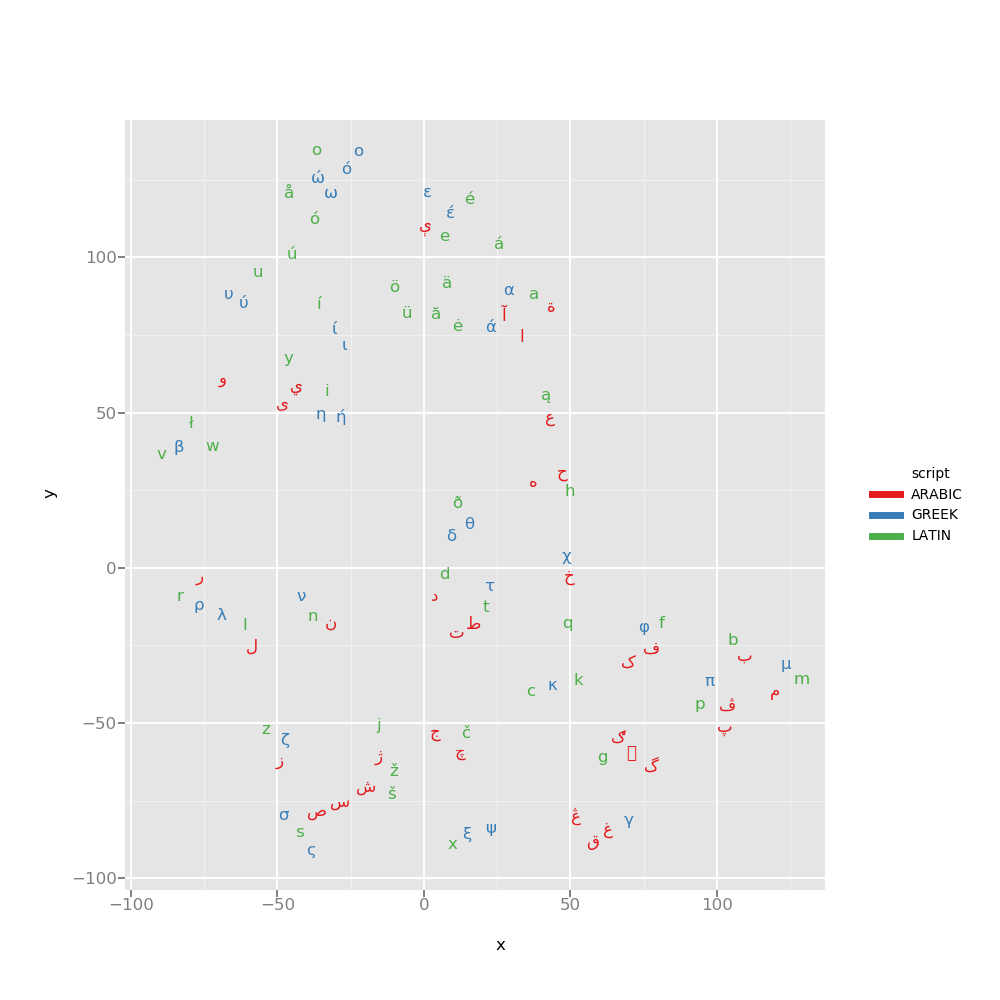
\includegraphics[scale=0.68]{Figures/latin-greek-arabic}
\caption{t-SNE projection of grapheme embeddings learned by \textsc{LangF-All} for graphemes from the Latin, Greek, and Arabic scripts. Greek and Arabic graphemes were included if they occurred at least 50 times in the training data, and Latin graphemes were included if they occurred at least 1000 times. The plot for the \textsc{LangID-All} data was very similar. Prior to performing t-SNE, embeddings were reduced to 40 dimensions with PCA. Perplexity was set to 10 and t-SNE was run for 2000 iterations.}
\label{figure:grapheme-tsne}
\end{figure}

%Understanding the grapheme embedding space could have important applications because many NLP systems are not robust to input in non-standard writing systems. In many languages that are written in other scripts, text is often romanized in informal settings such as text messages. A few works have looked into processing of romanized text, for example for Urdu \citep{irvine2012processing} and Arabic \citep{tobaili2016arabizi}. The \textsc{LangID} and \textsc{LangF} models put all graphemes in the same vector space regardless of script, so it would be interesting to see if they tend to locate graphemes near their equivalents in other alphabets. If they do, this suggests that g2p could be

%The Arabic example in Figure \ref{table:tokens} suggests that the models likely learn similar representations for analogous characters from different scripts. The model comes up with a somewhat reasonable Arabic pronunciation of a Latin alphabet string, even though the model received no training on data in the Latin alphabet. One 


\subsection{Phoneme Embeddings}
In addition to learning grapheme embeddings on the source side, the models learn phoneme embeddings on the target side. As is shown in Figure \ref{table:phonemes}, these do seem to show certain regularities. The voiced bilabial stop \textipa{/b/}, for example, is located closest to other bilabial sounds, the voiceless aspirated alveolar stop \textipa{/t\super h/} is located closest to voiceless stops at nearby places of articulation, and so on. This could be useful knowledge because the phoneme space is sparse, even though the model is shared across all languages: of the 464 phonemes present in the \textsc{LangID-All} and \textsc{LangF-All} training data, more than half of them occur less than 50 times and 73 occur only once. Accurate embeddings cannot be learned for such phonemes from training data alone. Any insight into how the phoneme space organizes itself could therefore help to estimate embeddings for these infrequent phonemes.

Similarly to the grapheme embeddings, I constructed t-SNE plots for the phoneme embeddings, which are shown in Figure \ref{figure:phoneme-tsne}. As can be seen, phonemes tend to cluster in ways that make sense phonologically. Vowels and consonants are mostly in separate clusters, and symbols that indicate tone are separate from both. Within the consonants, several natural classes can be observed: nasals are close to each other, labial sounds are close together, and so on. Within these clusters, some patterns can be seen as well: high vowels are close to other high vowels, for example. Consonants tend to associate based on a combination of place and manner of articulation, and not so much based on voicing: generally voiced and voiceless pairs, such as \textipa{/k/} and \textipa{/g/}, tend to be quite close. This observation aligns well the fact that allophones may differ in voicing in many languages. In German, for example, voiced stops (i.e. \textipa{/b/}, \textipa{/d/}, \textipa{/g/}) become voiceless (i.e. \textipa{/p/}, \textipa{/t/}, \textipa{/k/}) at the end of a word. This would lead to distributional similarity between these voiced-voiceless pairs. An allophone between a voiceless stop and a nasal, for example, would be less likely.

This apparent relationship between learned phoneme embeddings and articulatory facts could guide future research into parameter sharing. The \textsc{LangID} and \textsc{LangF} models use a form of hard parameter sharing in which a phoneme shares the same embedding across all languages. But the embeddings learned here suggest that phoneme embeddings can at least partially be shared \emph{between} phonemes. Possibly embeddings could be learned not the phonemes themselves, but rather for lower-level phenomena, such as place and manner of articulation. Such data is present in sources such as Phoible \citep{phoible}. One could also try a soft sharing architecture similar to the one suggested for the graphemes. In that case, Phoible could be leveraged to weight how much parameters should be shared between phonemes, based on the similarity of their articulatory vectors.

\begin{figure}
\centering
\small
\begin{tabular}{c|c}
\textbf{Phoneme} & \textbf{Closest phonemes} \\
\hline
\textipa{b} & \textipa{p\super h}, \textipa{B}, \textipa{F} \\
\textipa{@} & \textipa{\~a}, \textipa{\u{e}}, \textipa{W} \\
\textipa{t\super h} & \textipa{t:}, \textipa{\:t}, \textipa{\|[t} \\
\textipa{x} & \textipa{X}, \textipa{G}, \textipa{\textcrh} \\
\textipa{y} & \textipa{y:}, \textipa{Y}, \textipa{I} \\
\textipa{\*r} & \textipa{R\super G}, \textipa{\|[r}, \textipa{\;R} \\
\end{tabular}
\caption{Selected phonemes and the most similar phonemes, measured by the cosine similarity of the embeddings learned by the \textsc{LangID-All} model}
\label{table:phonemes}
\end{figure}

\begin{figure}
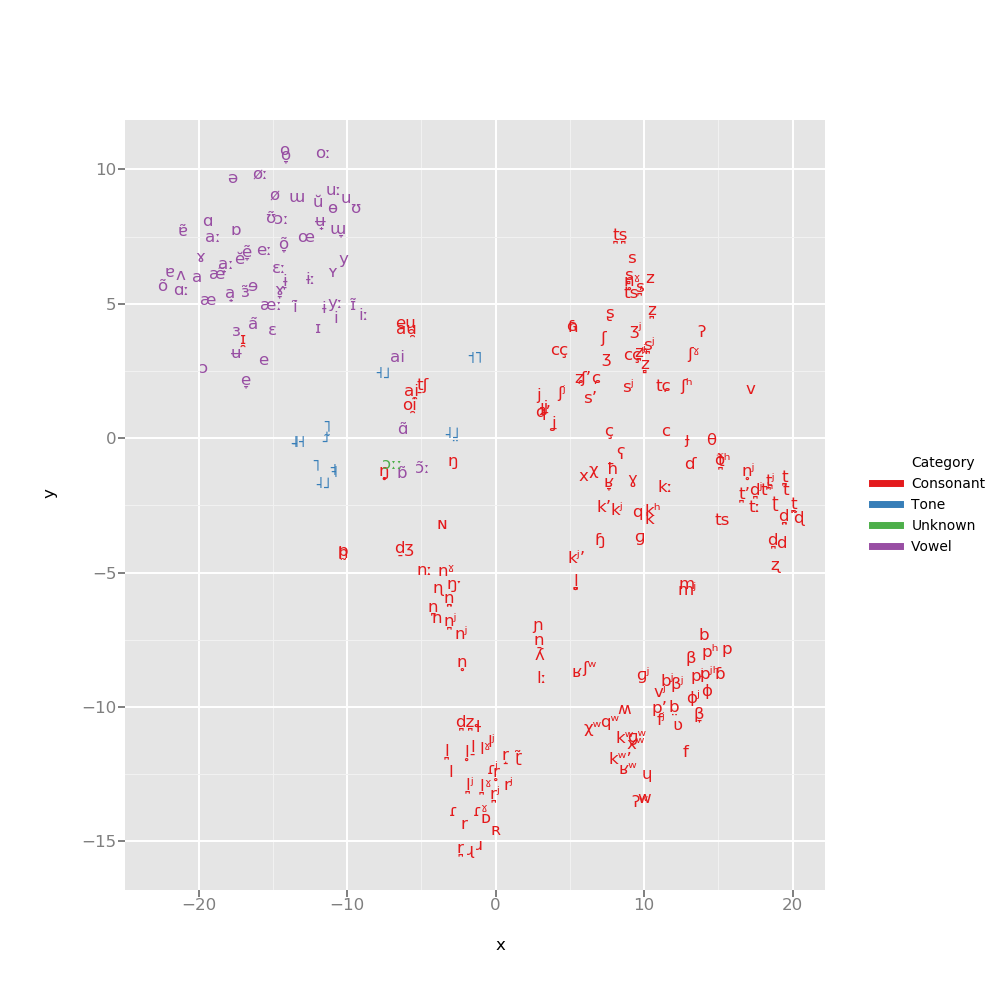
\includegraphics[scale=0.68]{Figures/langf-phonemes-smart-label}
\caption{t-SNE projection of phoneme embeddings for phonemes that occurred at least 50 times in the training data. Embeddings were reduced to 40 dimensions with PCA before applying t-SNE. Perplexity was set to 25 and t-SNE was run for 2000 iterations or until error failed to improve for 300 iterations.}
\label{figure:phoneme-tsne}
\end{figure}

\subsection{Language Embeddings}
Given the interesting structure present in the grapheme and the phoneme embeddings, it would be interesting to see if any patterns can be observed for the language embeddings. These kinds of embeddings have already been studied in a few works. \cite{ostling2017continuous} performed hierarchical agglomerative clustering on the language embeddings learned for their multilingual character-level language modeling task and found that languages often tended to cluster in a way that resembled genetic relationships. Other works \citep{malaviya17emnlp,bjerva2017tracking} have used language representations as features for typological prediction; this will be considered in Section \ref{typo-pred}.

The \textsc{LangID} and \textsc{LangF} models embed the languages differently: in the \textsc{LangID} models, the language is represented with a source-side token in the embeddings in the same space as the graphemes. As is shown in Figure\todo{make}, the grapheme and language embeddings are very clearly separated in the 

The \textsc{LangF} and \textsc{LangID} models also learn vectors that represent languages. Feature and token representations of the source language are both beneficial to performance, and therefore it would be useful to analyze and evaluate them to find out where the benefit comes from. A better understanding may suggest better ways to learn good language embeddings and directions for future research. A first pass at this analysis would be to visualize the language embeddings.



In contrast to \citeauthor{ostling2017continuous}'s results, the language embeddings learned by\todo{what about LangF?} \textsc{LangID-All} did not appear to show any genetic or geographic relationships\todo{check this out again}.

Instead, you can discuss how the languages separate from the graphemes for LangID

%Therefore, it would be difficult to estimate the embedding for an unseen language, or to ``borrow'' the language ID token of a similar language. A more promising way forward is to find a model that uses an externally constructed typological representation of the language.

%it would be useful to understand the structure of the space in which these tokens are embedded. Developing an understanding of this embedding space gives insight into the structure of the neural network and could allow embeddings to be more accurately estimated for languages that lack sufficient training data.



%One possible way to do so is with tokens that identify something other than the language, such as typological features about the language's phonemic inventory. This could enable better sharing of resources among languages. Such typological knowledge is readily available in databases like Phoible and WALS for a wide variety of languages. It would be interesting to explore if any of these features is a good predictor of a language's orthographic rules.

%Previous work has considered the structure and predictive power of distributed representations of languages \citep{ostling2017continuous,malaviya17emnlp}. I further this analysis by applying the language representations learned by \textsc{LangID-All}.

As \textsc{LangID-All} represents the language with an ordinary source-side token, a first step to analysis is to find out whether language embeddings are easy to distinguish from grapheme embeddings, which are located in the same space. In order to analyze the space, I applied t-distributed stochastic neighbor embedding (t-SNE) \citep{maaten2008visualizing} to \textsc{LangID-All}'s source-side embedding matrix for 2000 iterations with a perplexity of 50. Types that occurred less than 500 times in the training set were excluded because it was difficult to learn useful embeddings for them. The resulting plot is shown in Figure \ref{figure:l-g-tsne}.

\begin{figure}
\begin{center}
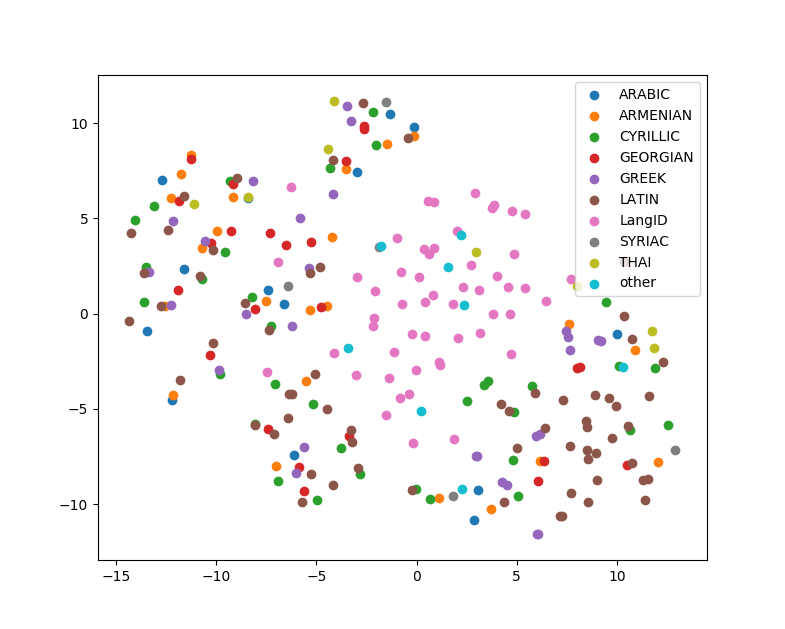
\includegraphics[scale=0.7]{Figures/lang-grapheme-500count-50-no-pca}
\end{center}
\caption{t-SNE projection of language and grapheme embeddings that occur at least 500 times in the \textsc{LangID-All} training data.}
\label{figure:l-g-tsne}
\end{figure}

As one might expect, the various language embeddings tend to be clustered in one region, distinct from the grapheme embeddings. The next question to ask is whether there are any patterns to observe within the language embeddings.\todo{plot, and try hierarchical stuff too}

\section{Embeddings for Typological Prediction}
\label{typo-pred}
\cite{bjerva2017tracking} used \citeauthor{ostling2017continuous}'s trained vectors for multilingually-trained part-of-speech taggers for Uralic languages. They additionally used these vectors as input for a typological prediction task which showed that the vectors encoded some typological facts. In a similar vein, \cite{malaviya17emnlp} used language representations learned by a many-to-English neural machine translation system for typological classification.

\subsection{Graphemes}
How accurately can you predict writing system?\todo{not really typological, though}

\subsection{Phonemes}

\subsection{Languages}

